\documentclass[12pt]{article}
\usepackage{fullpage}
\usepackage{graphicx}
\usepackage{amsmath,amsthm,amsfonts,amssymb}
\usepackage{amsmath}
\usepackage{algpseudocode,algorithm}
\usepackage{csquotes}
\usepackage[hidelinks]{hyperref}
\MakeOuterQuote{"}

\title{ML Algorithms Explained}
\author{Chenshu Liu}

\renewcommand{\listfigurename}{Figures}
\newcommand{\subsubsubsection}[1]{\paragraph{#1}\mbox{}\\}
\setcounter{secnumdepth}{3}
\setcounter{tocdepth}{4}

\begin{document}
\maketitle
\thispagestyle{empty}
\tableofcontents
\listoffigures
\thispagestyle{empty}
\newpage

\section{KNN}
\setcounter{page}{1}
KNN is the abbreviation of K Nearest Neighbors.
\begin{figure}[htbp]
\begin{center}
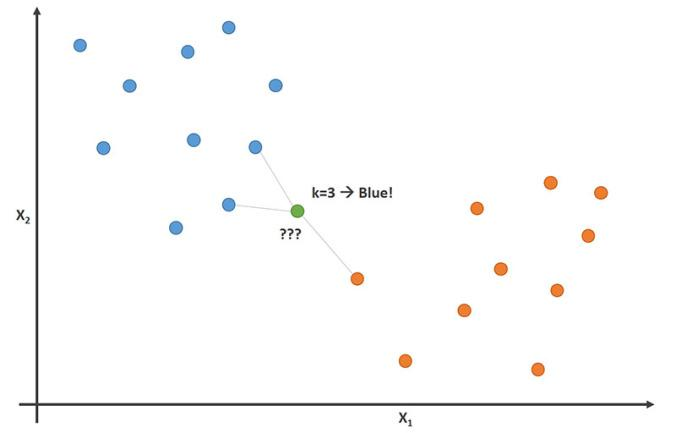
\includegraphics[width = 0.7\textwidth]{Images/KNN.jpeg}
\caption{KNN}
\label{KNN}
\end{center}
\end{figure}

\subsection{Process of KNN}
The process of determining the classification of the sample is:
\begin{enumerate}
	\item Find k (\textit{defined by user}) nearest neighbors of the sample point (\textit{e.g. the green point in Figure 1})
	\item Calculate the euclidean distance of the neighbor points (\textit{e.g. the blue and orange points in Figure 1}) from the sample points
	\item Since we already know the categories that the neighbor points belong to, we can use the \textbf{majority of the neighbor category} as the classification for the sample point (e.g. in the case of Figure 1, since two of the three points are blue, the sample point, i.e. the green point, is classified as blue)
\end{enumerate}
\newpage

\section{Linear Regression}
Linear regression is used to predict continuous values using the approximation formula $\hat{y} = wx + b$
\begin{figure}[htbp]
\begin{center}
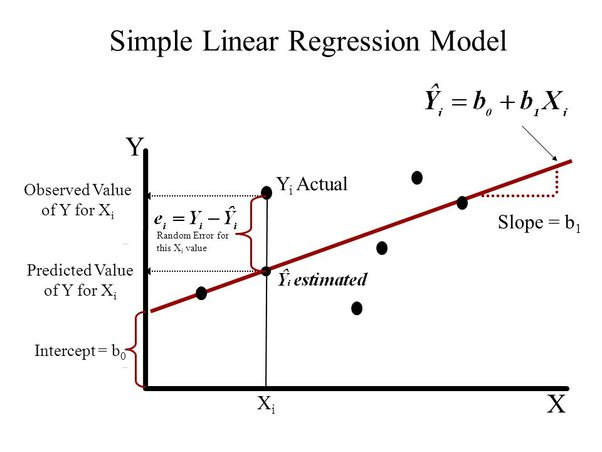
\includegraphics[width = 0.6\textwidth]{Images/Linear Regression.jpeg}
\caption{Linear Regression}
\label{default}
\end{center}
\end{figure}
\subsection{Math Logic Behind Linear Regression}
To find the optimal values of the weight w and intercept b, we introduce MSE to evaluate the error of prediction for some w and b. MSE is calculated as follows:
$$MSE = J(w, b) = \frac{1}{N}\Sigma_{i=1}^n(y_i - (wx_i + b))^2$$
Then, we use \textbf{gradient descent} to find the optimal set of $(w, b)$ that minimizes the partial derivates of MSE:
$$J'(w, b) = \begin{bmatrix} \frac{\partial f}{\partial w} \\ \frac{\partial f}{\partial b} \end{bmatrix} = \begin{bmatrix} \frac{1}{N}\Sigma -2x_i(y_i - (wx_i + b))\\ \frac{1}{N}\Sigma -2(y_i - (wx_i + b))\end{bmatrix}
$$
Gradient descent is an iterative process that iterates the calculation until the local minimum is reached. In this case, since we have two parameters $(w, b)$, we are conducting gradient descent in a two-dimensional space. After every iteration, we will update the parameters in the following way:
$$w = w - \alpha \cdot dw$$
$$b = b - \alpha \cdot db$$
\newpage

\section{Logistic Regression}
Logistic regression is a binary classification algorithm.
\begin{figure}[htbp]
\begin{center}
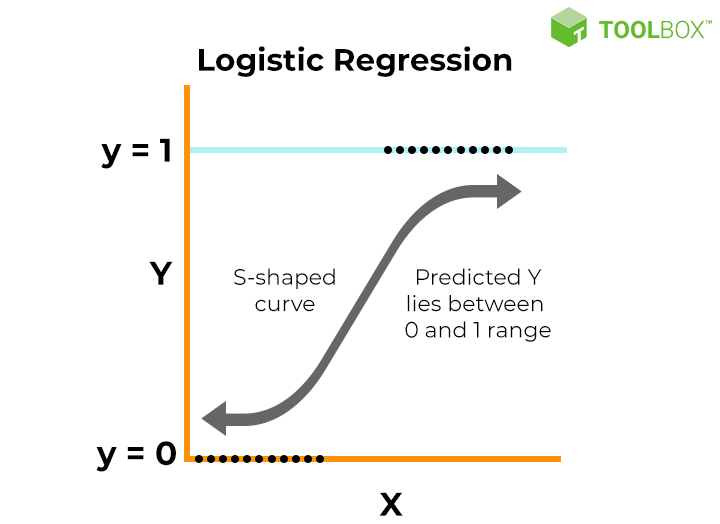
\includegraphics[width = 0.7\textwidth]{Images/Logistic Regression.png}
\caption{Logistic Regressiont}
\label{default}
\end{center}
\end{figure}

\subsection{Math Logic Behind Logistic Regression}
In linear regression, we model the behavior of the data using linear function to predict continuous values. In logistic regression, we want to predict binary outcomes, thus we will use a sigmoid function $s(x) = \frac{1}{1 + e^{-x}}$. And, for the prediction, we have $\hat{y} = h_{\theta}(x) = \frac{1}{1 + e^{-wx+b}}$. Similar to the process of finding optimal parameters for linear regression function, we also use gradient descent to find the best set of values for $(w, b)$ that provides the best prediction performance. The cost function, \textbf{cross entropy} is:
$$J(w, b) = J(\theta) = \frac{1}{N}\Sigma_{i=1}^n[y^ilog(h_{\theta}(x^i) + (1-y^i)log(1 - h_{\theta}(x^i))]$$
The gradient descent procedure is the same as those from the linear regression section.
\newpage

\section{Naive Bayes}
Naive Bayes is a classification algorithm that is achieved through the Bayes Theorem.
\begin{figure}[htbp]
\begin{center}
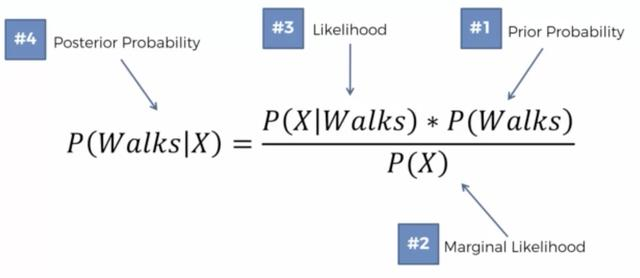
\includegraphics[width = 0.7\textwidth]{Images/Naive Bayes.jpeg}
\caption{Naive Bayes}
\label{default}
\end{center}
\end{figure}

\subsection{Math Logic Behind Naive Bayes}
\subsubsection{Bayes Theorem}
Bayes Theorem:
$$P(A|B) = \frac{P(B|A)\cdot P(A)}{P(B)}$$
In our case, using X to predict for y:
$$P(y|X) = \frac{P(X|y)P(y)}{P(X)}$$
\subsubsection{Assumption}
Though in real life cases, all features are rarely independent, but the assumption of all features being mutually independent still proves to be effective:
$$P(y|X) = \frac{P(x_1|y)\cdot P(x_2|y)\cdot \dots \cdot P(x_n|y)\cdot P(y)}{P(X)}$$
Where:
\begin{enumerate}
	\item Prior probability $P(y)$ is just the frequency
	\item Class conditional probability follows the gausian distribution: $P(x_i|y) = \frac{1}{\sqrt{2\pi \sigma  y^2}}\cdot
exp(-\frac{(x_i - \mu_y)^2}{2\sigma  y^2})$
\end{enumerate}
\subsubsection{Naive Bayes Algorithm}
Then, the classification is performed by selecting the class with the highest probability:
$$y = argmax_yP(y|X) = argmax  y\frac{P(x_1|y)\cdot P(x_2|y)\cdot \dots \cdot P(x_n|y)\cdot P(y)}{P(X)}$$
$$y = argmax_yP(x_1|y)\cdot P(x_2|y)\cdot \dots \cdot P(x_n|y)\cdot P(y)$$
Because all the probabilities are values between 0 and 1, and multiplying them may lead to the product being a very small number. Thus, in order to prevent overflow, we can apply logarithm to the product:
$$y = argmax_ylog(P(x_1|y)) + log(P(x_2|y)) + \dots + log(P(x_n|y)) + log(P(y))$$
\newpage

\section{Perceptron}
Perceptron is a simplified version of a biological neuron.

\subsection{Background of Perceptron Model}
The neuron in the biological system receives inputs through dendrites and generates one response (\textit{i.e. output}) through the axon. In the perceptron model, we can express the pipeline of information processing using a linear function $y = w^Tx + b$ where $w$ is the weight assigned to each input node and $b$ is the bias. 

\begin{figure}[htbp]
\begin{center}
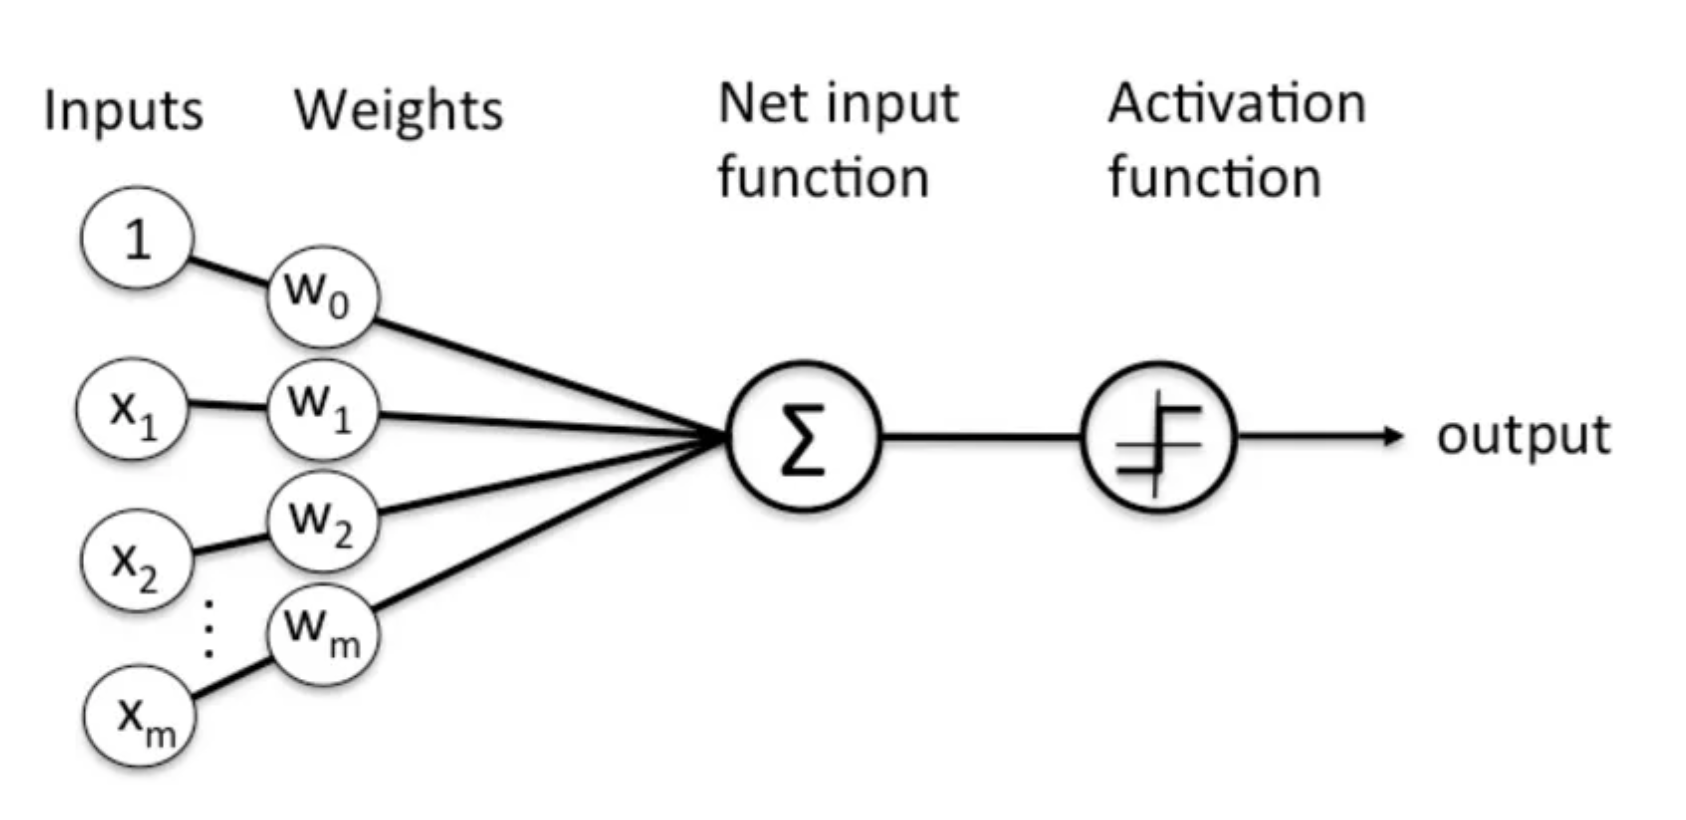
\includegraphics[width = 0.7\textwidth]{Images/Perceptron.png}
\caption{Perceptron}
\label{default}
\end{center}
\end{figure}

\subsection{Perceptron Model}
In Figure 5, we can see that after the input and weights are manipulated, an activation function is called. In the case of perceptron, it is simple the unit step function that becomes significant only when the value reaches certain threshold.\\
\\
Thus, we can summarize the pipeline as $\hat{y} = g(f(w, b)) = g(w^Tx + b)$, and through the training process, we can update the parameters using the perceptron update rule, such that for each training sample $x_i$:
\begin{enumerate}
	\item $w := w + \Delta w$
	\item $\Delta w := \alpha \cdot (y_i - \hat{y_i})\cdot x  i$
	\item learning rate $\alpha$ is between [0, 1]
\end{enumerate}

\subsection{Math Logic Behind Perceptron}
During the dynamic update of the weights, the weights are adjusted to better match the prediction with the actual value. So, the reason why there is a $(y_i - \hat{y  i})$ term is that:
\begin{enumerate}
	\item When the predicted $\hat{y  i}$ is greater than the actual $y  i$, the weight update $\Delta w$ has a negative value, reducing the weight in the new iteration
	\item When the predicted $\hat{y  i}$ is less than the actual $y  i$, the weight update $\Delta w$ has a positive value, increasing the weight in the new iteration
	\item In sum, the weights are pushed towards positive or negative target class in cases of misclassification  
\end{enumerate}
NOTE: perceptron only works for linearly separable classes (i.e. classes that can be separated using a linear function). For further improvements, the activation function can be changed accordingly (i.e. instead of using the unit step function, we can use functions like the sigmoid function)
\newpage

\section{SVM}

\subsection{Background}
SVM is the abbreviation for support vector machine. The aim of SVM is to find a linear decision boundary, also known as hyperplane if considering higher dimensions, that best separates the data to perform classification.\\
\\
The definition of the best hyperplane is that the distance of the data points from different classes to the hyperplane is maximized (\textit{Figure 6}). Also, the separation needs to be clear (i.e. the two classes need to be on opposite sides of the hyperplane) so that the linear model satisfies the following conditions:
\begin{itemize}
	\item $w\cdot x - b = 0$
	\item $w\cdot x_i - b \geq 1$ if $y_i = 1$ or belongs to class 1
	\item $w\cdot x_i - b \leq -1$ if $y_i = -1$ or belongs to class -1
	\item Summarizing point 2 and 3, we have $y_i(w\cdot x_i + b) \geq 1$. If all sample points satisfies the condition, then the separation by the hyperplane is perfect
\end{itemize}

\begin{figure}[htbp]
\begin{center}
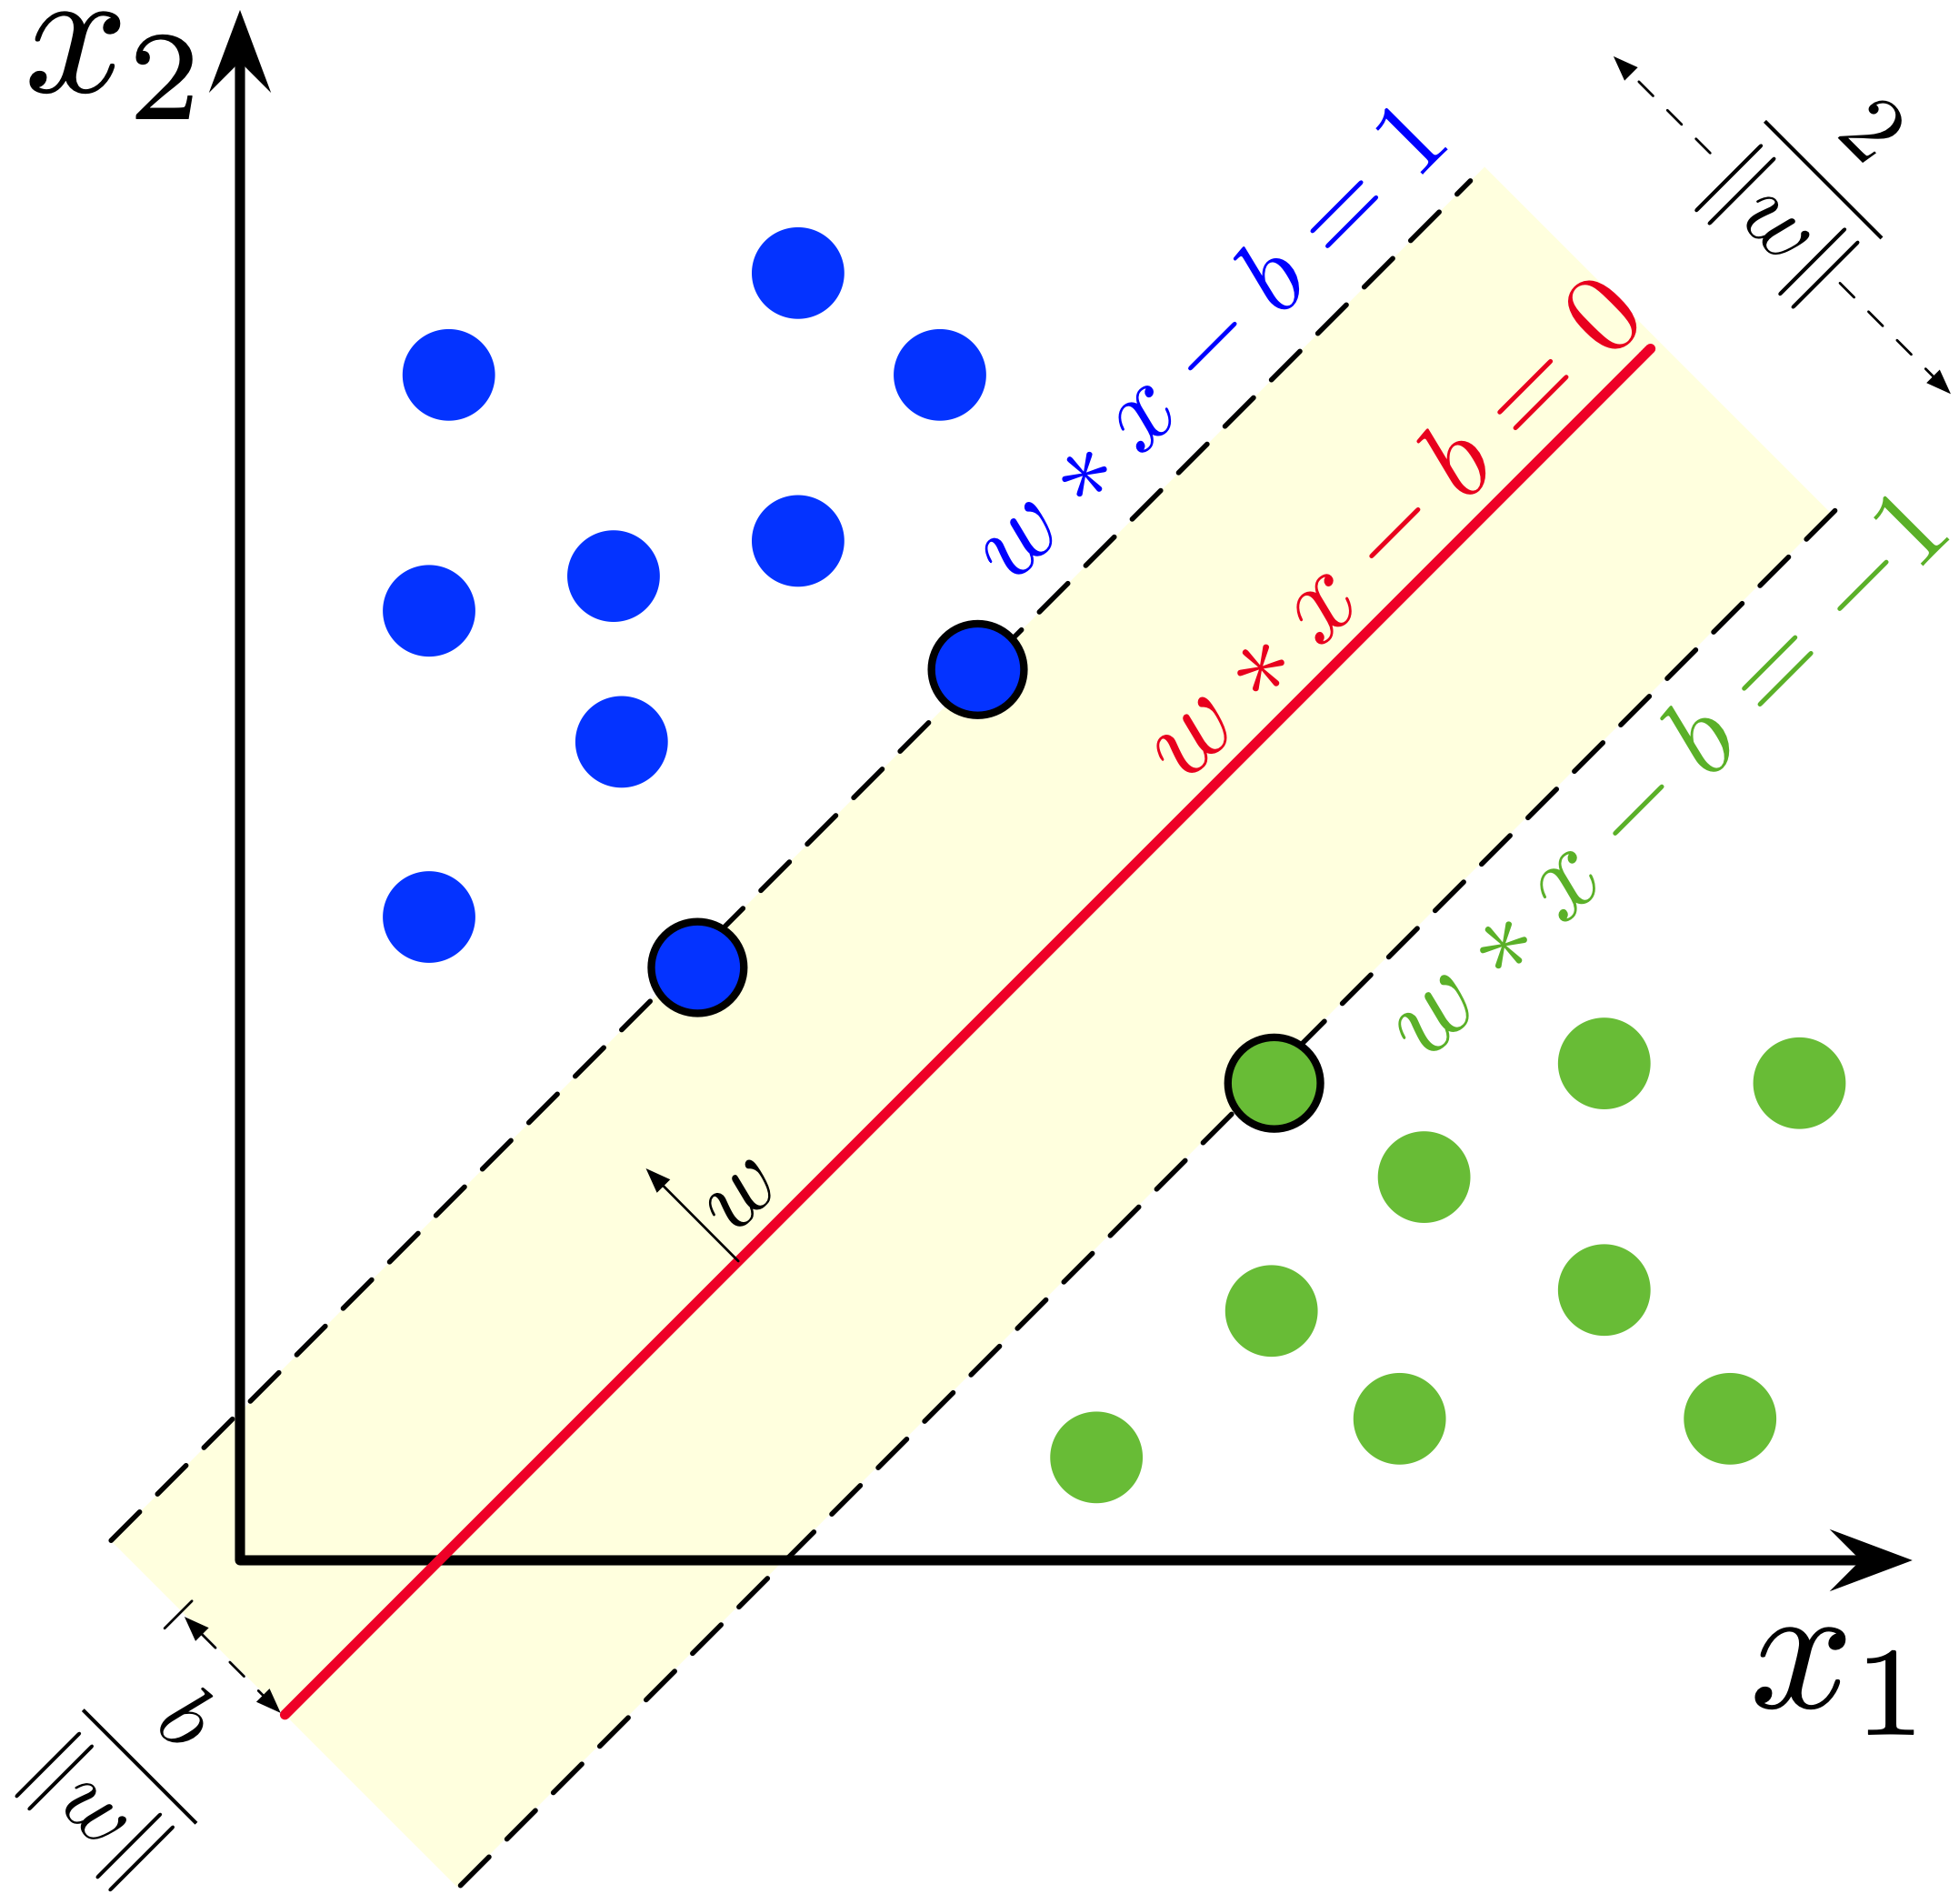
\includegraphics[width = 0.5\textwidth]{Images/SVM.jpeg}
\caption{SVM}
\label{default}
\end{center}
\end{figure}

\subsection{Math Logic Behind SVM}
\subsubsection{Hinge Loss}
Using the conclusion that $y_i(w\cdot x_i + b) \geq 1$, we can further define the loss function, more specifically called the Hinge loss:
$$l = max(0, 1 - y_i(w\cdot x_i + b))$$
Since we know that if the classification is correct, $y_i(w\cdot x_i + b) \geq 1$, then when the classification is correct for a sample case, the maximum of the loss function is 0, indicating no loss. Otherwise, the loss is defined by the expression $1 - y_i(w\cdot x_i + b)$. Thus, we can summarize the possible cases of the loss as:
$$l =
\begin{cases}
0 & \text{if } y\cdot f(x) \geq 1\\
1 - y\cdot f(x) & \text{otherwise}
\end{cases}$$
\subsubsection{Cost Function}
While formatting the cost function, we not only consider the loss function, but also take into account of the margin of separation. Recall that the goal of SVM is to find the best separating hyperplane, that is, to have the distance from data points to the hyperplane to be maximized. The margin, according to geometry, is $\frac{b}{||w||}$. Thus, to maximize the margin, we need to minimize $||w||$. So, we can generalize the cost function as:
$$J = \lambda ||w||^2 + \frac{1}{n}\Sigma_{i=1}^{n}max(0, 1 - y_i(w\cdot x_i + b))$$
Thus, there are two cases for the cost function:
\begin{itemize}
\item When the classification is correct (i.e. $y_i\cdot f(x) \geq 1$)
\begin{itemize}
	\item $J_i = \lambda ||w||^2$
	\item $\frac{\partial J_i}{\partial w_k} = 2\lambda w_k$
	\item $\frac{\partial J_i}{\partial b} = 0$
\end{itemize}
\item When the classification is incorrect
\begin{itemize}
	\item $J_i = \lambda ||w||^2 + 1 - y_i(w\cdot x_i + b)$
	\item $\frac{\partial J_i}{\partial w_k} = 2\lambda w_k - y_i \cdot x_i$
	\item $\frac{\partial J_i}{\partial b} = y_i$
\end{itemize}
\end{itemize}

Finally, the update rule is similar to previous gradient descent parameter updates:
\begin{itemize}
	\item $w = w - \alpha\cdot dw$
	\item $b = b - \alpha\cdot db$
\end{itemize}
\newpage

\section{Decision Tree}
Decision tree is a tree like classification algorithm that classifies data through numerous nodes of criteria.

\subsection{Math Logic Behind Decision Tree}
\subsubsection{Entropy \& Information Gain}
The decision tree has many nodes, there are criteria at each node to separate data points to different categories. The way to determine what feature to be put in which decision node is determined by the calculating the change in entropy, and whichever node can contribute to the highest information gain (IG) can be placed at more superior decision node. Entropy is defined as:
$$E = -\Sigma p(X)\cdot log_2(p(X))$$
where $p(X) = \frac{\# x}{n}$

\subsection{Stopping Criteria}
Of course, we cannot let the tree to continuously grow, otherwise it would lead to overfitting. Thus, during the construction of decision trees, we will set stopping criteria such as:
\begin{itemize}
	\item Maximum depth
	\item Minimum samples at a node
	\item No more class distribution in node
\end{itemize}

\subsection{Decision Making}
The choice of decision node is determined through calculating the information gain of every possible criteria. The criteria that results in the highest information gain is then assigned as the most superior decision node.

\subsection{Example}
For example, in Figure 7:
\begin{figure}[h]
\begin{center}
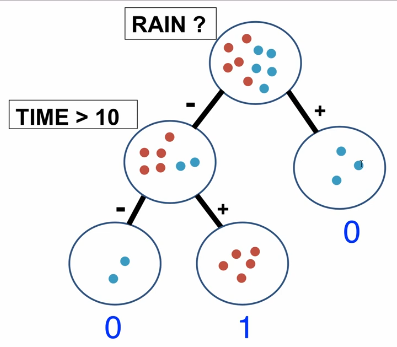
\includegraphics[width = 0.5\textwidth]{Images/Decision Tree.png}
\caption{Decision Tree}
\label{default}
\end{center}
\end{figure}
\subsubsection{First Iteration}
The original set has ten data points, 5 are 0's and 5 are 1's, $S = [0, 0, 0, 0, 0, 1, 1, 1, 1, 1]$. So we can calculate the entropy as:
$$E = -\frac{5}{10}\cdot log_2(\frac{5}{10}) - \frac{5}{10}\cdot log_2(\frac{5}{10}) = 1$$

\subsubsection{Second Iteration}
\textbf{Entropy}\\
After the first decision node, the original data is separated into two clusters, with one cluster having $S_1 = [0, 0, 0, 0, 0, 1, 1]$ and the other having $S_2 = [1, 1, 1]$. Thus, the entropy of the two clusters can be calculated as:
$$E(S_1) = -\frac{5}{5+2}\cdot log_2(\frac{5}{5+2}) - \frac{2}{5+2}\cdot log_2(\frac{2}{5+2}) \approx  0.863$$
$$E(S_2) = 0 \text{ because the cluster only has one category, }p(X)\text{ is 1, and }log_2(p(X))\text{ is 0}$$
\textbf{Information Gain}\\
The information gain (IG) can be calculated as:
$$IG = E(parent) - [\text{weighted average}]\cdot E(children)$$
$$IG = E(S) - [(\frac{7}{10})\cdot E(S_1) + (\frac{3}{10})\cdot E(S_2)]$$
$$IG = 1 - [\frac{7}{10}\cdot 0.863 + \frac{3}{10}\cdot 0] = 0.395$$
\newpage

\section{Random Forest}
Random forest is an aggregation of numerous decision trees.

\begin{figure}[htbp]
\begin{center}
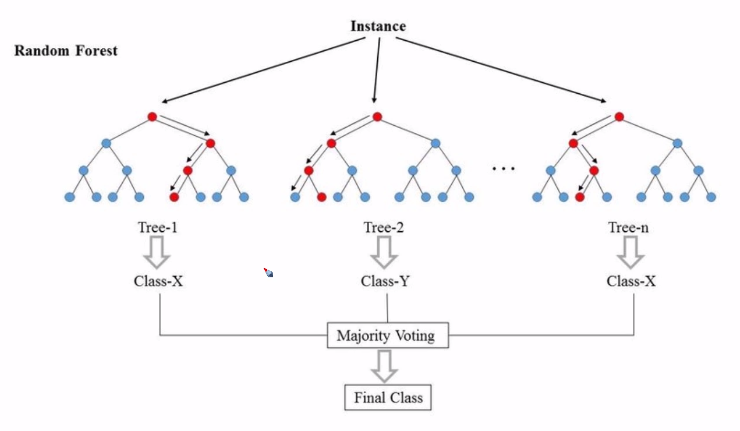
\includegraphics[width = 0.7\textwidth]{Images/Random Forest.png}
\caption{Random Forest}
\label{default}
\end{center}
\end{figure}


\subsection{Logic Behind Random Forest}
Random forest is constructed by combining multiple decision trees, each tree having random subset of the training data, then classification is made by taking the majority vote.

Random forest has the following advantages over decision trees:
\begin{itemize}
	\item Avoid overfitting
	\item Have higher prediction accuracy
\end{itemize}
\newpage

\section{PCA}
\subsection{Purpose of PCA}
PCA stands for principle component analysis that finds a new set of dimensions through a transformation of axes such that:
\begin{itemize}
	\item The transformed features are linearly independent (i.e. orthogonal)
	\item The projected points have maximum spread (i.e. maximum variance)
\end{itemize}

\begin{figure}[htbp]
\begin{center}
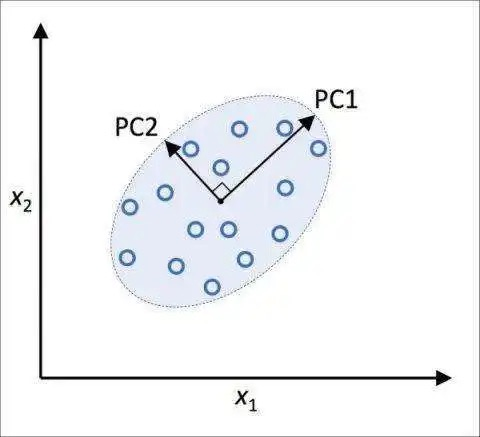
\includegraphics[width = 0.5\textwidth]{Images/PCA.jpeg}
\caption{PCA}
\label{default}
\end{center}
\end{figure}

\subsection{PCA Algorithm}
PCA can be conducted through the following steps:
\begin{enumerate}
	\item Calculate Cov(X, X)
	\item Calculate the eigenvectors and eigenvalues of the covariance matrix
	\item Sort the eigenvectors according to their eigenvalues in decreasing order to show their ability to explain about the variance
	\item Choose the first k eigenvectors that will be the new dimensions (discard eigenvectors that are less significant in explaining the data variance)
	\item Transform the original n dimensional data points into k dimensions using the new dimension (i.e. project onto the new set of dimensions)
\end{enumerate}
\newpage

\section{K-Means}
K-means is an unsupervised learning algorithm that cluster a dataset into k different clusters according to the distance to the nearest mean

\begin{figure}[htbp]
\begin{center}
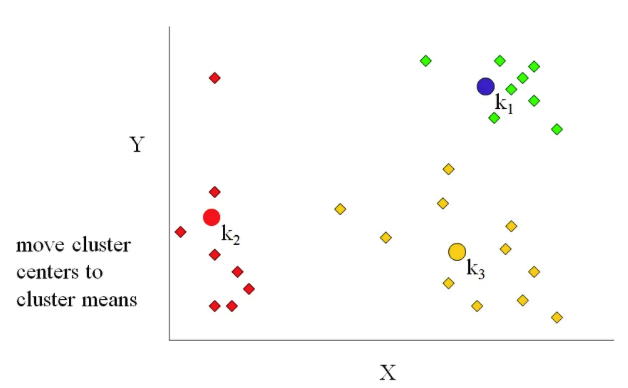
\includegraphics[width = 0.7\textwidth]{Images/K-Means.png}
\caption{K-Means}
\label{default}
\end{center}
\end{figure}


\subsection{Logic Behind K-Means}
\subsubsection{Euclidean Distance}
The euclidean distance is calculated using the formula (i.e. the euclidean distance between two feature vectors):
$$d(p, q) = \sqrt{\Sigma(p_i - q_i)^2}$$
\subsubsection{K-Means Algorithm}
K-means is achieved through iterative optimization:
\begin{enumerate}
	\item Cluster centers were initialized randomly at first
	\item Repeat until the clustering result converges (i.e. the clustering result does not change anymore)
	\begin{enumerate}
		\item Update the cluster labels according to the euclidean distance (i.e. assign points to the nearest cluster centers)
		\item Update the cluster centers (i.e. centroids) by setting the new centroids to the mean of each cluster
    	\end{enumerate}
\end{enumerate}
\newpage

\section{AdaBoost}
\subsection{AdaBoost vs. Random Forest}
AdaBoost functions in a similar fashion as Random Forests, they all conduct numerous separate decision processes and then aggregate the decision results and choose the majority vote.\\
\\
However, AdaBoost is different from Random Forest in the following ways:
\begin{itemize}
	\item AdaBoost uses stumps, or weak learners (classifiers that can only use one feature variable for classification at a time, unlike decision trees that are used in random forest that can use several feature variables in one decision process), or weak classifiers, and assign different weights to the decision made by each stump then aggregate all the decision results to make the final classification.
	\item Each decision tree planted in the Random Forest is independent from other, recall that we randomly assign samples to the decision trees when implementing Random Forest. However, the stumps in AdaBoost are sequential (i.e. the performance of the first stump determines how the second stump is made, and the performance of the second stump influences how the third stump is made, etc.)
\end{itemize}

\begin{figure}[htbp]
\begin{center}
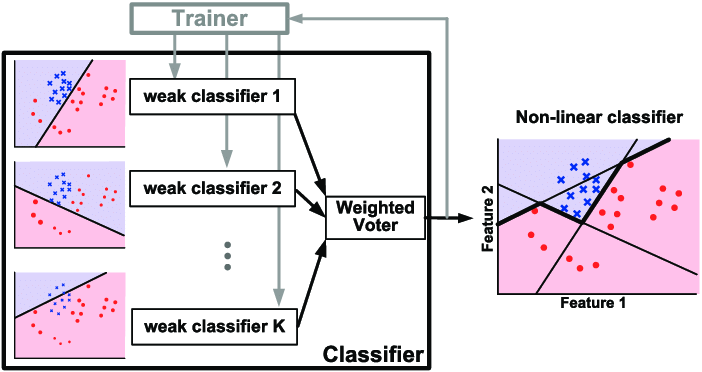
\includegraphics[width = 0.7\textwidth]{Images/AdaBoost.png}
\caption{AdaBoost}
\label{default}
\end{center}
\end{figure}

\subsection{Math Logic Behind AdaBoost}
\subsubsection{Error}
$$\epsilon_t = \frac{\text{number of misclassifications}}{samples} = \frac{\text{number of misclassifications}}{N} \text{ \textbf{Note}: only the first iteration}$$
In later iterations, if a sample is misclassified, we give it a higher weight to guide the next classification:
$$\epsilon_t = \Sigma_{miss}weights$$
If the error is higher than 0.5, then the classification will be flipped entirely

\subsubsection{Weights}
The weights for each sample is set to be $w_0 = \frac{1}{N}$, which makes sense because the error related to the first iteration is $\epsilon_t = \text{number of misclassifications}\cdot \frac{1}{N}$. However, as AdaBoost progresses, the weights also updates, according to the misclassification rates:
$$w = \frac{w\cdot exp(-\alpha\cdot y\cdot h(X))}{sum(w)}$$
where:
\begin{itemize}
	\item $\alpha$ is the accuracy of the classifier $\alpha = 0.5\cdot log(\frac{1-e_t}{e_t})$
	\begin{itemize}
		\item if $e_t \rightarrow 1$ (i.e. all the classifications are wrong), the weight will approach a really negative value to correct the classification to the opposite side
		\item if $e_t \rightarrow 0$ (i.e. all the classifications are correct), the weight will approach a really positive value to maintain the classification at the same side
		\item if $e_t \rightarrow 0.5$ (i.e. the classification is like flipping a coin with 50/50 chance), the weight will approach 0, which does not affect further stumps
    	\end{itemize}
	\item $h(X)$ is the prediction of t
\end{itemize}

\subsubsection{Prediction}
$$y = sign(\Sigma_t^T \alpha_t \cdot h(X))$$
\newpage

\section{LDA}

LDA stands for linear discriminant analysis. 

\begin{figure}[htbp]
\begin{center}
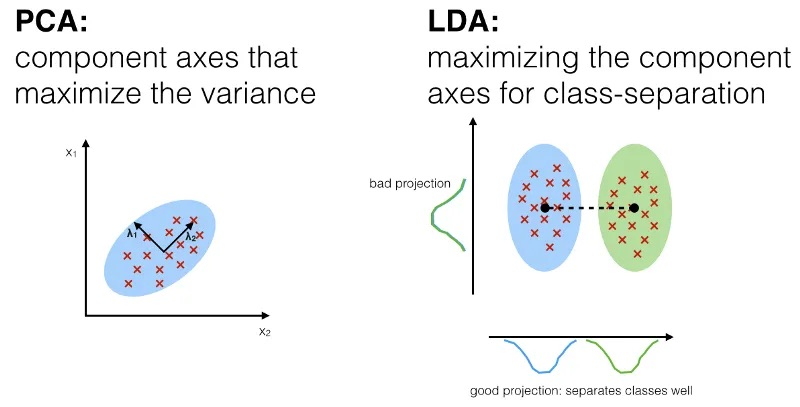
\includegraphics[width = 0.7\textwidth]{Images/PCA vs. LDA.jpeg}
\caption{PCA vs. LDA}
\label{default}
\end{center}
\end{figure}

\subsection{PCA vs. LDA}
It is similar to the PCA algorithm that can reduce dimension during data preprocessing. Both LDA and PCA's goal is to reduce the complexity of the features (i.e. project a dataset onto a lower-dimensional space with good class-separability)

LDA is different from PCA in the following ways:
\begin{itemize}
	\item PCA is an unsupervised learning algorithm while LDA is supervised (i.e. the label of each data point is known)
	\item PCA finds component axes that can maximize the variance among data points while LDA is not only trying to maximize variance among data points but is also trying to maximize the separation between multiple classes
\end{itemize}

\subsection{Math Logic Behind LDA}
Because LDA is interested in both within-class variance and between-class variance, we will consider the following:
\begin{itemize}
	\item Within-class Scatter Matrix
$$S_W = \Sigma_c S_c$$
$$S_c = \Sigma_{i \in c}(\bar{x_i} - \bar{x_c})(\bar{x_i} - \bar{x_c})^T$$
	\item Between-class Scatter Matrix
$$S_B = \Sigma_{i \in c}n_c\cdot (\bar{x_c} - \bar{x})(\bar{x_c} - \bar{x})^T$$
\end{itemize}
Then, to solve for the new dimensions that can maximize both the between and within class variances, we will solve for the eigenvalue and eigenvector of $S_W^{-1}S_B$

\subsection{LDA Algorithm}
Procedure to construct LDA algorithm is:
\begin{enumerate}
	\item Calculate $S_W$ and $S_B$
	\item Calculate the eigenvalues and eigenvectors of $S_W^{-1}S_B$
	\item Sort the eigenvectors according to the eigenvalues in decreasing order
	\item Choose the first k eigenvectors so that the dimension is reduced to k
	\item Transform the original n dimensional data points into k dimensions using dot product
\end{enumerate}

\end{document}
